\documentclass[crop,tikz]{standalone}
\usepackage{tikz}
\usetikzlibrary{calc}
\usetikzlibrary{positioning}
\begin{document}
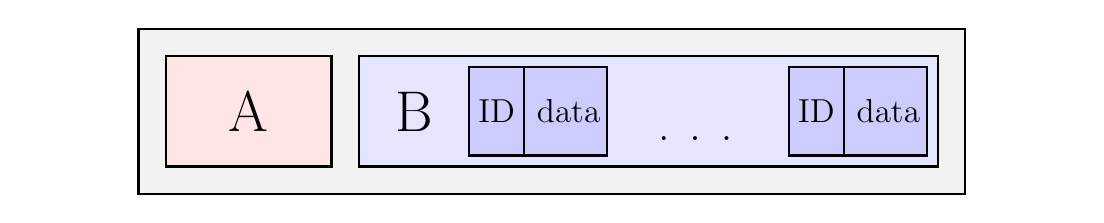
\begin{tikzpicture}[scale=0.07,rotate=0]
	
	%Background
	\draw[draw=white, fill=white] (0,0) rectangle (190,30);
		
	%Frame
	\draw[thick, draw=black, fill=gray!10] (20,0) rectangle (170,30);

	%Segments
	%A
	\draw[thick, draw=black, fill=red!10] (25,5) rectangle (55,25);
	\node at (40,15) {\huge A};

	%B
	\draw[thick, draw=black, fill=blue!10] (60,5) rectangle (165,25);
	\node at (70,15) {\huge B};
	
	%B1
	\draw[thick, draw=black, fill=blue!20] (80,7) rectangle (90,23);
	\draw[thick, draw=black, fill=blue!20] (90,7) rectangle (105,23);
	\node at (85,15) {\large ID};
	\node at (98,15) {\large data};
	
	\node at (121,10) {\LARGE . . .};
	
	%Bn
	\draw[thick, draw=black, fill=blue!20] (148,7) rectangle (163,23);
	\draw[thick, draw=black, fill=blue!20] (138,7) rectangle (148,23);
	\node at (143,15) {\large ID};
	\node at (156,15) {\large data};
	
\end{tikzpicture}
\end{document}